\documentclass{standalone}
\usepackage{textcomp}
\usepackage{pgfplots}
\begin{document}
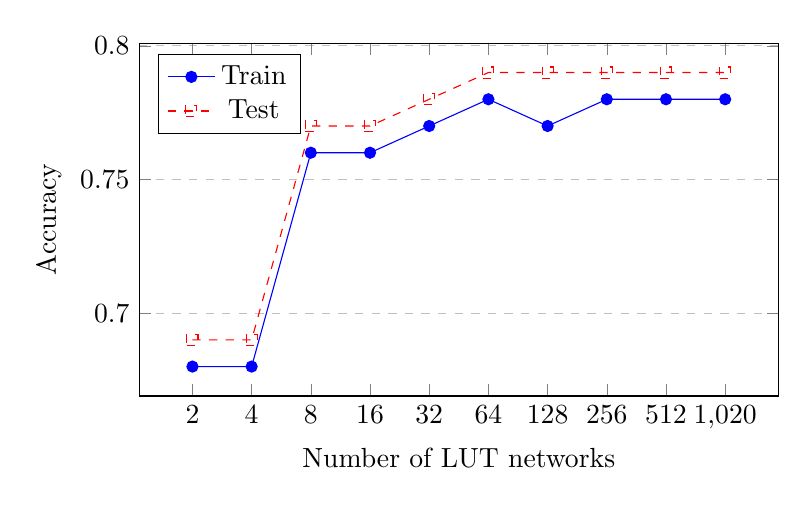
\begin{tikzpicture}
\begin{axis}[
    %title={Real data},
    width=0.8\textwidth,
    height=0.5\textwidth,
    xlabel={Number of LUT networks},
    ylabel={Accuracy},
    %xmin=1, xmax=17,
    %ymin=0.44, ymax=1.1,
    xtick={2,4,8,16,32,64,128,256,512,1024},
    %ytick={0.5,0.6,0.7,0.8,0.9,1.00},
    legend pos=north west,
    ymajorgrids=true,
    grid style=dashed,
    xmode=log,
    log ticks with fixed point,
]

\addplot[
    color=blue,
    mark=*,
    ]
    coordinates {
        (2,0.68)(4,0.68)(8,0.76)(16,0.76)(32,0.77)(64,0.78)(128,0.77)(256,0.78)(512,0.78)(1024,0.78)
    };
    \addlegendentry{Train}

\addplot[
    color=red,
    mark=square,
    dashed,
    ]
    coordinates {
        (2,0.69)(4,0.69)(8,0.77)(16,0.77)(32,0.78)(64,0.79)(128,0.79)(256,0.79)(512,0.79)(1024,0.79)
    };
    \addlegendentry{Test}

\end{axis}
\end{tikzpicture}
\end{document}
